\begin{problem}{육각타일미로탈출기}{standard input}{standard output}{1 second}{256 megabytes}

윤수는 파티로 가려는 도중 악랄한 종현에 의해 육각타일미로에 빠지게 되었다. 미로는 일정한 크기의 정육각형 타일로 구성된 $N$행 $M$열의 격자 형태로 이루어져 있다. 같은 열에 위치한 두 칸을 비교했을 때, 짝수 번째 행의 칸은 홀수 번째 행의 칸보다 반 칸 오른쪽에 위치해 있다. $N$, $M$이 각각 $4$, $7$일 때의 그림은 아래와 같다.
\begin{center}
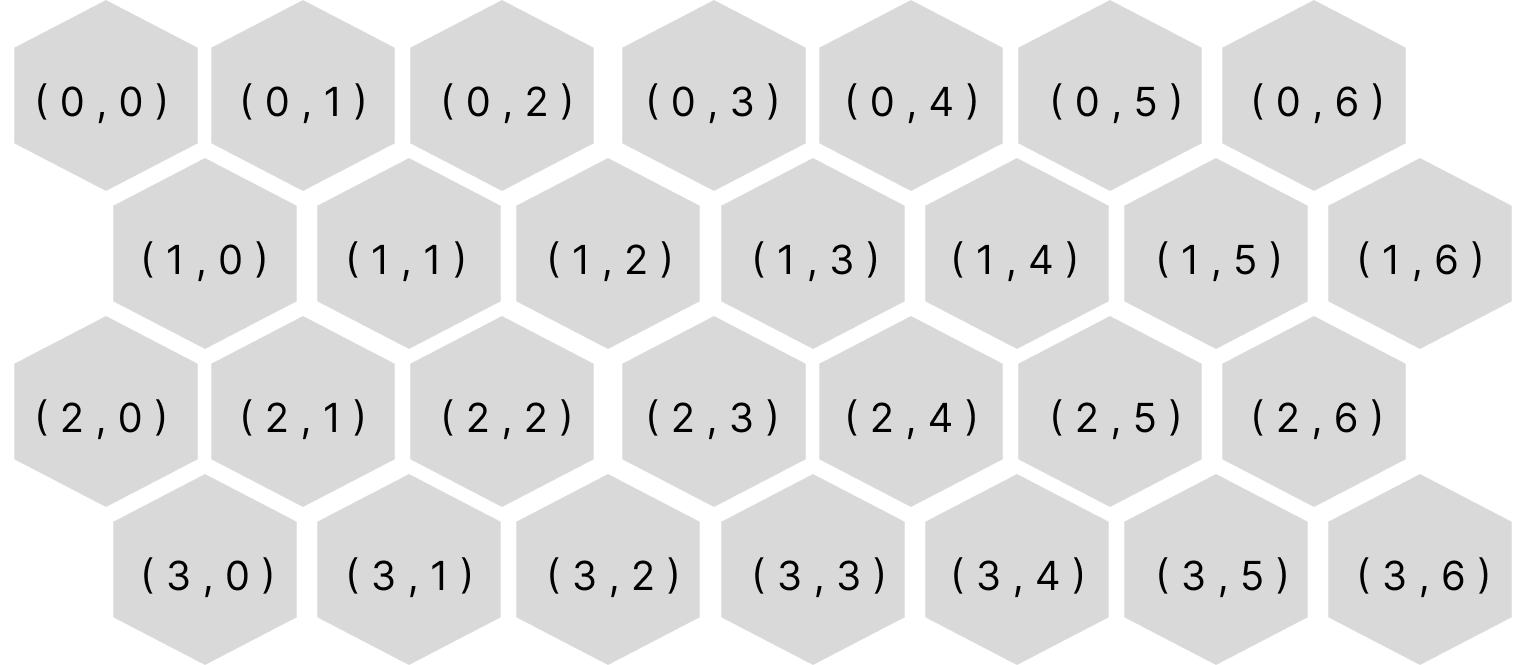
\includegraphics[bb=0 0 100 200]{Group1.png}
\end{center} 

윤수는 항상 $(0,0)$에서 시작하며 탈출구는 항상 $(N-1, M-1)$에 존재한다. 종현은 윤수의 탈출을 막기 위해 $K$개의 장애물을 타일 위에 두었다. 육각타일 위에서는 인접한 타일로 이동할 수 있지만 장애물이 있는 타일로는 이동할 수 없다. 두 육각형 타일이 하나의 변을 공유한다면 서로 인접하다고 한다.  

윤수는 서둘러 파티를 가고 싶기 때문에 미로를 탈출할 수 있는 최단 경로를 찾으려고 한다. 최단 경로는 육각타일미로에서 탈출구까지 가장 적은 개수의 타일을 지나는 경로를 말하는데, 이때 시작하는 타일은 포함하지 않고 탈출구가 있는 타일은 포함해서 센다. 윤수가 탈출구에 도달하기 위한 최단 경로의 타일의 개수를 알아보자. 단, 탈출구에 도달할 수 없을 경우 $-1$을 출력한다. 

\InputFile
첫 번째 줄에 $N$, $M$, $K$가 공백으로 구분되어 주어진다.$(2 ≤ N, M ≤ 1000;$ $0 ≤ K ≤ N×M-2)$

다음 $K$개의 줄에 장애물의 위치 $Y_k$$(0 ≤ Y ≤ N-1)$, $X_k$$(0 ≤ X ≤ M-1)$ 가 공백으로 구분되어 주어진다. 두 장애물의 위치가 같은 경우는 주어지지 않고 시작점과 탈출구에는 장애물이 존재하지 않는다.


\OutputFile
윤수가 탈출구에 도달하기 위한 최단 경로의 타일의 개수를 출력한다. 단, 탈출구에 도달할 수 없을 경우 $-1$을 출력한다.

\Examples

\begin{example}
\exmpfile{example.01}{example.01.a}%
\exmpfile{example.02}{example.02.a}%
\exmpfile{example.03}{example.03.a}%
\end{example}

\end{problem}

